\documentclass[a4paper]{article}

\begin{document}
\title{Osborne 1 floppy drive emulator}
\date{July 2024}
\author{Archie Halliwell \and Lennart Leufgens \and Jun Muta \\
John Monash Science School}
\maketitle

\subsection{Problems}

The first problem we ran into was that a capacitor in the Osborne 1
exploded when it was first plugged in---the capacitor had absorbed
moisture over the years and this caused it to heat up and
explode---but this was easily fixed by replacing the capacitor with a
modern one.

The first board we had made turned out to be too big, and collided with
the power connector on the Osborne's logic board, so we had to design a second
version, for which we used more SMD components, enabling us to shrink
it to less than half the size.

\begin{figure}
  \centering
  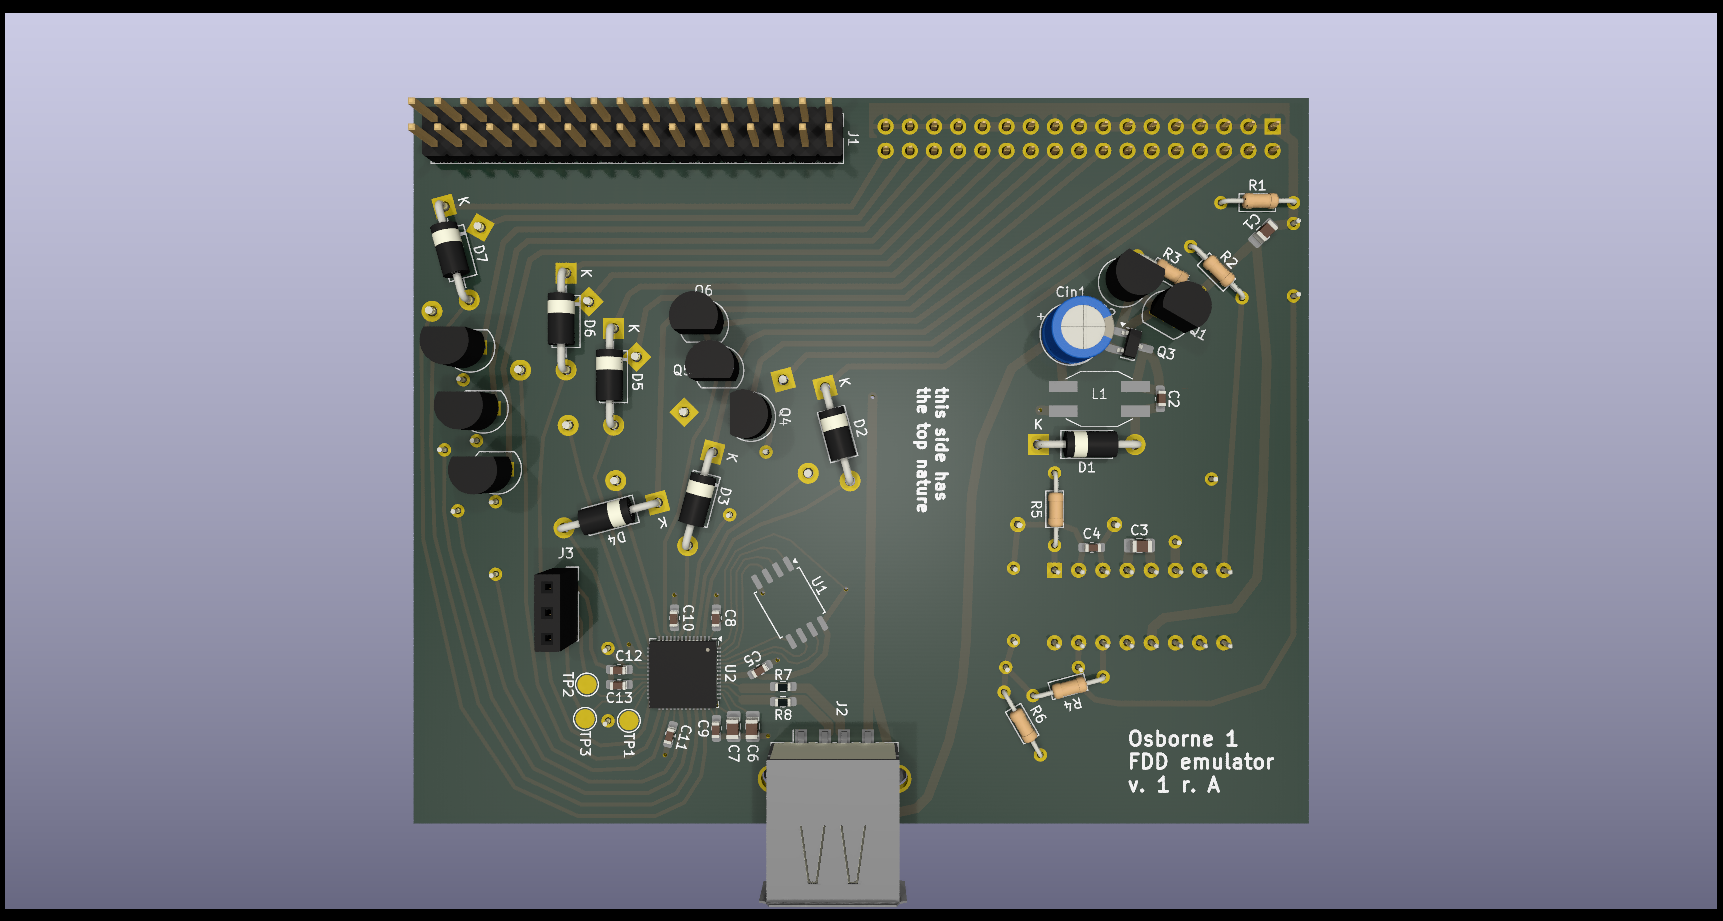
\includegraphics[height=5cm]{pcb-v1}
  \caption{Render of first version of PCB}
\end{figure}

\begin{figure}
  \centering
  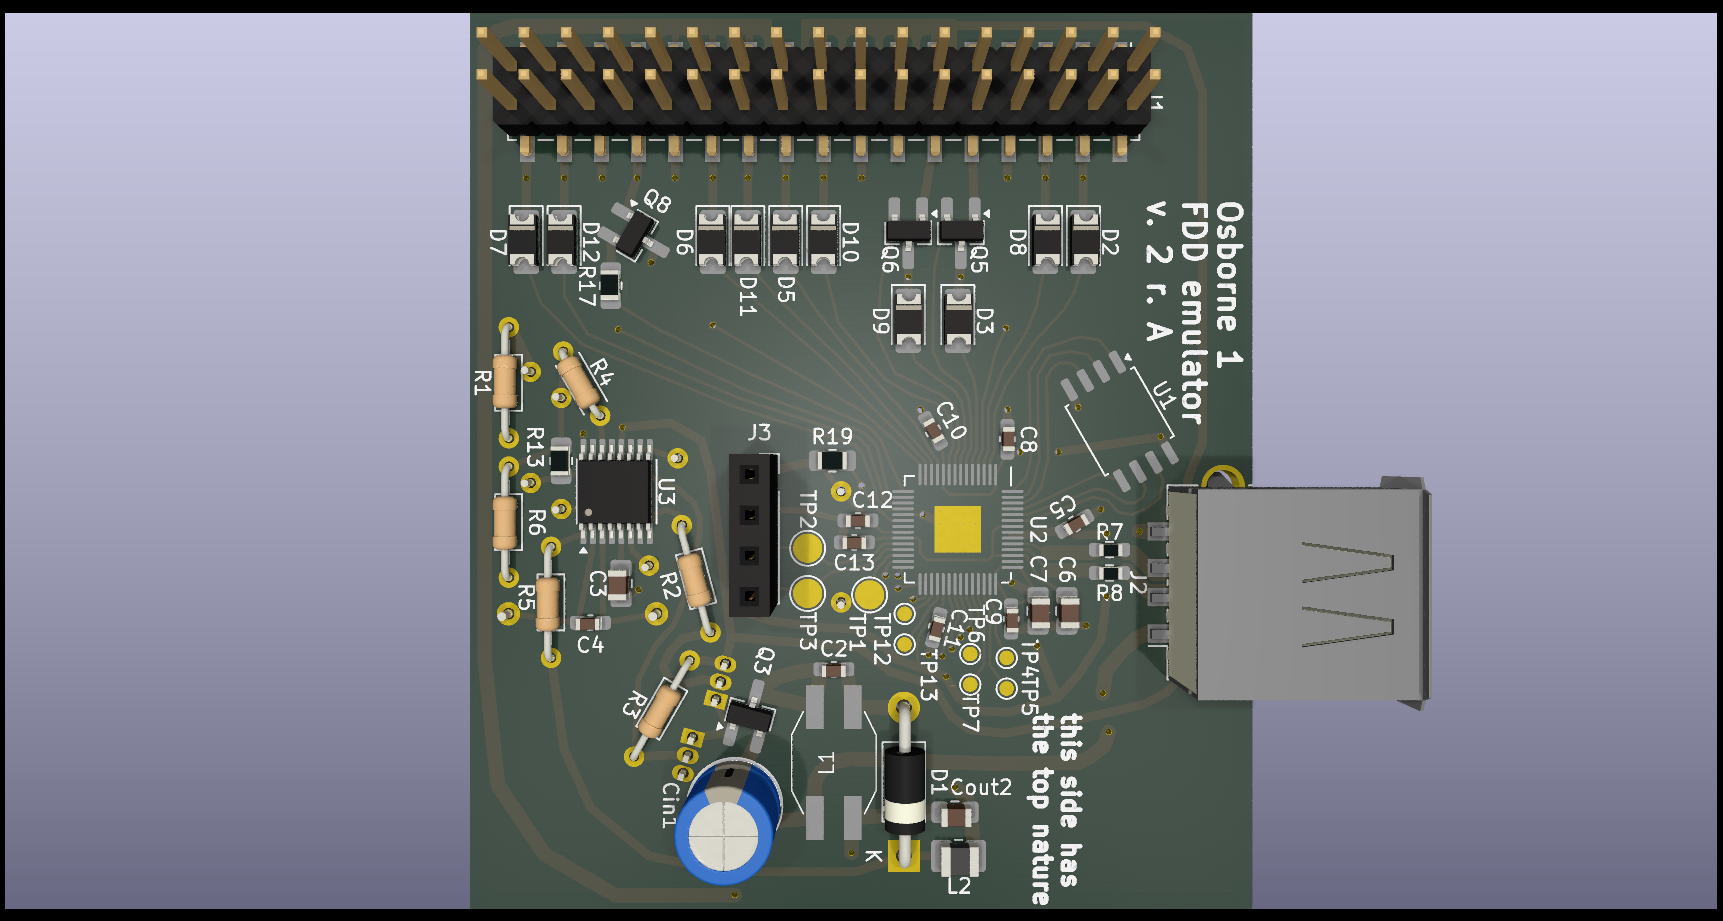
\includegraphics[height=5cm]{pcb-v2}
  \caption{Render of second version of PCB}
\end{figure}

Once we managed to get the RP2040 to run using the clock provided by
the Osborne 1, the increased power draw caused the tiny common-mode
choke in our power supply to saturate, causing excessive power draw
and insufficient voltage. To fix this we replaced it with a hand-wound
inductor we made earlier.

\begin{figure}
  \centering
  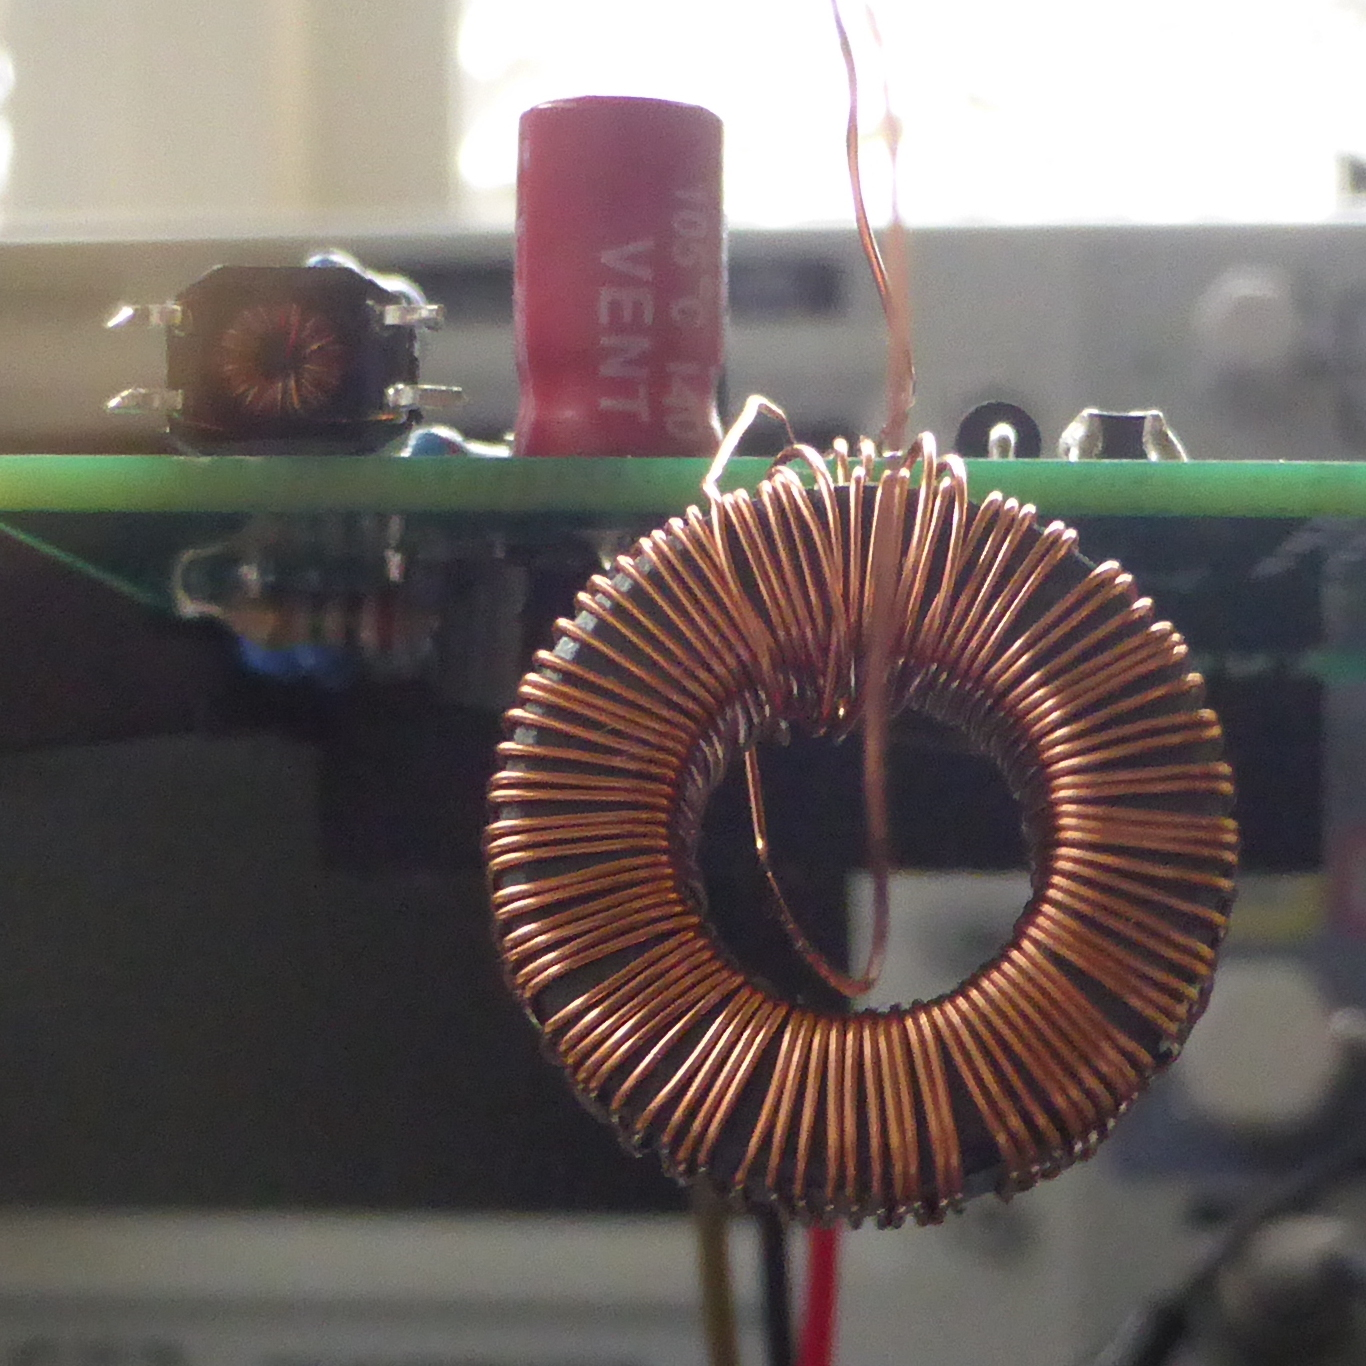
\includegraphics[height=5cm]{inductors}
  \caption[Inductors]{SMD common-mode choke (left) and hand-wound
    coupled inductors (right)}
\end{figure}

\begin{figure}
  \centering
  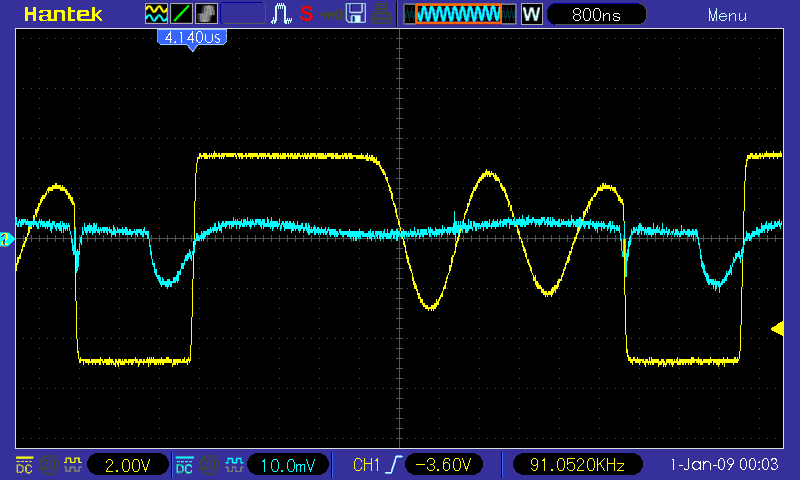
\includegraphics[height=3.5cm]{pic_25_1}\hfill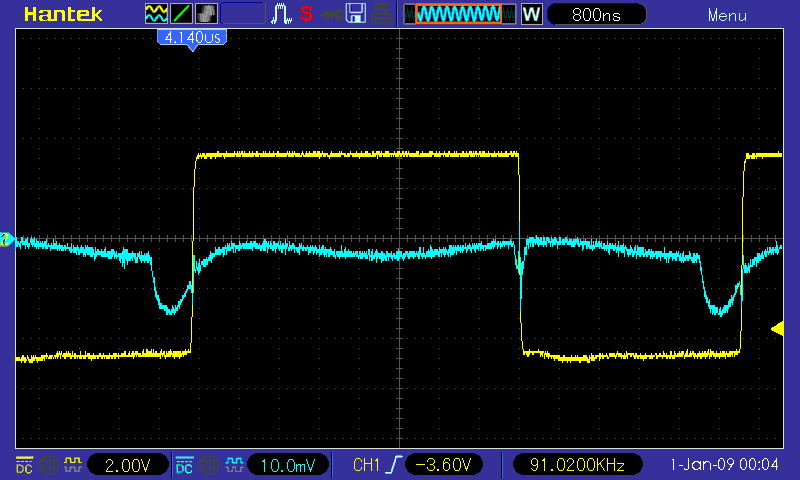
\includegraphics[height=3.5cm]{pic_25_4}
  \caption[Voltage and current traces with handwound inductors]{Diode
    anode voltage vs. time (yellow) and voltage across \qty{0.1}{\ohm}
    shunt (blue) with hand-wound inductors---On left under light load (in
    DCM) and on right under high load (in CCM)}
\end{figure}

\end{document}